% TODO fix citation style
% TODO make printbibliography work

\documentclass[10pt,a4paper]{article}
\usepackage[utf8]{inputenc}
\usepackage[english]{babel}

\usepackage{csquotes}
\usepackage{hyperref}
\usepackage{graphicx}
\usepackage{amsmath}

\usepackage{sty/usecases}
\usepackage{sty/arduinoListing}

\usepackage[
backend=biber,
style=alphabetic,
citestyle=authoryear 
]{biblatex}

\addbibresource{jabref.bib}

\title{Armoniacs: Automatized Aquaponics with Arduino}
\author{Guilherme Alcarde Gallo \and Christian Esteve Rothenberg \and Edmundo Roberto Mauro Madeira}

% define \req command to label requirements in description environment
\makeatletter
\newcommand{\req}[1]{
  \def\@currentlabel{R#1}\label{req#1}
  \textbf{R#1}
}
\makeatother

\begin{document}

\maketitle

\newpage

\tableofcontents

\newpage

\section{Introduction}
\label{sec:introduction}
\subsection{Motivation}
Basically,
the automation purpose is to save labor and add more security,
precision and velocity to tasks that formerly were made by humans or other animals.

If someone wonder about the reason for automating things,
this person probably doesn't pay attention about living in modern civilizations.
When one walks on the sidewalk,
one can see vehicles parked on the road,
these are automated things,
because saves the labor of walking to distant places,
via the electronic management of several components,
such as acceleration,
fuel measurement,
injection,
breaking with ABS technology etc.
But not only cars are automated.
The microwave,
airplanes and elevators are automated objects which are used frequently.

Generally, 
an automation project is composed by a microcontroller, 
electronic devices and a variable number of sensors.
The former is the main component,
which is responsible to manage the system by reading the input from the latter,
and then process what to do,
so it can send signals to electronic devices to accomplish the system's goal.
This processing is made with programming,
a programmer can install the code inside the microcontroller,
which will execute the program when turned on.
So it is presupposed that the programmer will align the program with the system's intention.

\subsubsection{Context}
When someone builds an Aquaponics system,
one needs to manage it everyday,
since there is a plenty of work to do for maintaining the system work,
because it deals with living beings.
So it is a time wasting management,
with lots of repetitive tasks,
which one can be understood as periodic events.

Some of these tasks can be reliably automated,
together with others that involves problems that may occur during the system's growth.
For example, the fish feeding is a periodic event,
but the water's pH control is not a periodic event,
instead it is classified as an adverse event.

Basically this work is trying to decrease human intervention in an Aquaponics system via automatic management of adverse and periodic events,
in order to reduce the time wasted to take care of the system, 
as well as to make the management more reliable.


\subsection{Challenges}

\subsubsection{Without automation}
To build an Aquaponics system,
one needs to be precise and cautious when one makes the design of the project,
there are lots of requirements that need to be respected in order to make the Aquaponics work.
The most important requirements are strongly connected with equilibrium,
because we are dealing with a biological system.
For example,
the proportion between the fish tank and the plant's grow bed tank are vital to optimize.
If one gets the wrong proportion,
the system won't work,
both the fish and the plants will die precociously \cite{Leatherbury2014}.

Another problem is to distribute the byproducts of each medium to another one,
the main byproduct of the fish tank is ammonia,
if the concentration of the latter increases,
the fish will die by high toxicity,
hence this ammonia has to be delivered to the bacteria,
who will digest this substance via the nitrogen cycle,
producing nitrate.

As the final product are comestibles,
there is another concern: food toxicity.
One cannot use components made with materials that can cause water contamination,
because the fish and the plant will be contaminated as well.
So there is the need to use non-toxic elements in the system.
Besides there is also a high concern with the water source,
the water cannot be infected with pathogens that causes diseases,
like amoeba.

\subsubsection{With automation}
In order to automate an Aquaponics system,
one must take care with microelectronic components,
they have to be protected from water and humidity.

Second,
there is the need to use relays to add high current-drain devices,
like the submersible water pump,
which is essential to the system.
If this advise is ignored,
the microcontroller will be damaged.


\section{Objectives}
% Problem characterization and goals
\label{objectives}
Decrease human intervation in an Aquaponics system via automatic management of periodic events.
For example, the fish feeding is a periodic event,
but the water's pH control is not a periodic event,
instead it is classified as an adverse event.


\section{Theoretical Fundamentals}
\label{fundamentals}
\subsection{Background}
\subsection{Technologies}
\subsection{Related work}
\subsection{Conclusion}


\section{System Proposal}
\label{proposal}
\subsection{Approach}
\subsection{Use Cases}
%Sometimes it is a good idea to put domain objects in \texttt{}
%The template and the descriptions are based on the book Applying UML and Patterns: 
%An Introduction to Object-Oriented Analysis and Design and Iterative Development
%(3rd Edition) by Craig Larman.
\begin{usecase}

\addtitle{Water cycle control}{Template test} 

%Scope: the system under design
\addfield{Scope:}{System-wide}

%Level: "user-goal" or "subfunction"
\addfield{Level:}{User-goal}

%Primary Actor: Calls on the system to deliver its services.
\addfield{Actors:}{Microcontroller}

%Stakeholders and Interests: Who cares about this use case and what do they want?
\additemizedfield{Stakeholders and Interests:}{
	\item Stakeholder 1 name: his interests
	\item Stakeholder 2 name: his interests
}

%Preconditions: What must be true on start and worth telling the reader?
%\addfield{Preconditions:}{}
%when multiple
\additemizedfield{Preconditions:}{
    \item The Microcontroller must be installed in the system
    \item Water pump and the PWM module are working normally
} 

%Postconditions: What must be true on successful completion and worth telling the reader
\addfield{Postconditions:}
{
    The fish tank's water should be pumped to the vegetable media each quarter of an hour.
}
%when multiple
%\additemizedfield{Preconditions:}{}

%Main Success Scenario: A typical, unconditional happy path scenario of success.
\addscenario{Main Success Scenario:}{
	\item The Microcontroller executes a run cycle of 25\% in the PWM in a 1 hour period.
	\item The circuit sends this signal to a relay.
    \item The relay activates the water pump at a 15 minutes per hour rate with the adequate voltage.
}

%Extensions: Alternate scenarios of success or failure.
%\addscenario{Extensions:}{
	%\item[2.a] Invalid login data:
		%\begin{enumerate}
		%\item[1.] System shows failure message
		%\item[2.] User returns to step 1
		%\end{enumerate}
	%\item[5.a] Invalid subsriber data:
		%\begin{enumerate}
		%\item[1.] System shows failure message
		%\item[2.] User returns to step 2 and corrects the errors
		%\end{enumerate}
%}

%Special Requirements: Related non-functional requirements.
\additemizedfield{Special Requirements:}{
	\item R1: Operation Time Limit requirement
	\item second applicable non-functional requirement
}

% TODO: COOL Technology and Data Variations List: Varying I/O methods and data formats.
%\addscenario{Technology and Data Variations List:}{
	%\item[1a.] Alternative first action with other technology
%}

%Frequency of Occurrence: Influences investigation, testing and timing of implementation.
%\addfield{Frequency of Occurrence:}{}

%Miscellaneous: Such as open issues/questions
%\addfield{Open Issues:}{}

\end{usecase}


\subsubsection{Summary table}


\subsection{Requirements}
\subsection{Systems Architecture}

\subsection{Prototype Implementation and Project Decisions}
There are a lot of authors that have had experience with Aquaponics automation.
Most of them chooses Arduino or Raspberry Pi as the main microcontroller.

Two great reasons for the Arduino's usage are:
This work's author already has an Arduino UNO,
but not a Raspberry PI.
Besides the main reference of this work,
the Kretzinger's guide \cite{Leatherbury2014},
who has many years of experience with Aquaponics and its automation and he uses the Arduino as microcontroller.

The chosen components have been based in the references.

\subsection{Results and Rating}


\section{Implementation}
\label{implementation}
\subsection{Periodic Water Cycling Code}

%\minisec{Sketch 1: A flashing LED on a protoboard}

\begin{lstlisting}[style=Arduino, caption=Water Cycle First Code, label=lst:water1]
 /*  Emits a periodic signal one quarter per hour */

// Which pin is connected with the water pump?
const int waterPumpPIN = 4;

// Time intervals
// 15 min = 60e3 ms * 15 = 9e5 ms
const int fifteenMin = 900000;
const int fourtyFiveMin = 2700000;

void setup(){
  // Sets the waterPumpPIN as the output of the periodic signal
  pinMode(waterPumpPIN, OUTPUT);
}

void loop(){
  digitalWrite(waterPumpPIN, HIGH); // sets the signal to logical 1 ON
  delay(fifteenMin); // stay on high voltage for 15 minutes
  digitalWrite(waterPumpPIN, LOW); // sets the signal to logical 0 OFF
  delay(fourtyFiveMin); // stay on low voltage for 45 minutes
}
\end{lstlisting}

% Make a second code based on https://www.arduino.cc/en/Tutorial/BlinkWithoutDelay
\subsubsection{Reviewed Code}
A program that uses delay in the main loop to make timed actions is error-prone,
since the delay will be belated by the overhead of other operations located inside the main loop.
Moreover the Arduino will not detect any interruption during a delay,
so we need to use delays only when it is really necessary.

To make a better code and to improve the scalability of the automation for more use cases that needs to be precisely timed,
one needs to review the code to find another way to do periodic actions.
We used \cite{arduinoDelay} as a reference to remove the delay-based code from water cycling's code \ref{lst:water1}.
Given that Arduino only offers a functions that retrieve time in order of milliseconds,
the listing \ref{lst:wcReview} uses the millis() function.

\begin{lstlisting}[style=Arduino,
                    caption=Water Cycle Code without Delays,
                    label=lst:wcReview]

 /*  Emits a periodic signal one quarter per hour without using delay */

// Which pin is connected with the water pump?
const int waterPumpPIN = 4;

// State of the signal
int waterPumpState = LOW;

// Using unsigned variable to support more data
unsigned long previousMillis = 0; (*@ \label{lst:long} @*)

// Time intervals
// 15 min = 60 s * 15 = 9e3 s
const int fifteenMin = 9000;
unsigned long previousSeconds = 0;
// Milliseconds in one second
const int second = 1000;
// Seconds in one hour
const int hour = 3600;

void setup(){
  // Sets the waterPumpPIN as the output of the periodic signal
  pinMode(waterPumpPIN, OUTPUT);
}

void loop(){
  // Get current time in milliseconds
  unsigned long currentMillis = millis();

  // If a second passes
  if (currentMillis - previousMillis >= second) {
    // Store the last timestamp for the last second
    previousMillis = currentMillis;
    // Increment the number of seconds passed
    ++previousSeconds;
    // Reset each hour
    previousSeconds (*@\%= hour@*);
  }

  // For 15 minutes do
  if ( previousSeconds <= fifteenMin ) {
    digitalWrite(waterPumpPIN, HIGH); // sets the signal to logical 1 ON
  }
  // For other 45 minutes do
  else {
    digitalWrite(waterPumpPIN, LOW); // sets the signal to logical 0 OFF
  }
  
}
\end{lstlisting}

Note that we are storing the timestamps in a 32-bit variable at line \ref{lst:long},
so the overflow will occur in almost 50 days,
because the variable storage limit is $ ( 2^{32} -1 ) $ ms.
\begin{align}
    limit& = FFFF& limit+1& = 0000 \label{overflow}
\end{align}
The overflow phenomenon is showed in \eqref{overflow},
when 4 bytes can't afford to represent larger numbers anymore,
because all bits are set to 1.
If someone adds one to this limit,
the value turns to zero,
due to the 9th bit, or the carry, is ignored.

But there is a fancy property with this overflow that soothes this worry:
the subtraction of two timestamps will remain correct even if there is a overflow in those numbers,
given that the variable is unsigned.
\begin{align}
    time_A &=limit - 3\;milliseconds =FFFB  \label{timeA} \\ 
    time_B &= 10\;milliseconds =000A =limit + B  \label{timeB} \\ 
    time_B - time_A &= 000A - FFFB =000E =14\;milliseconds \label{difference}
\end{align}

For example,
$time_A$ \eqref{timeA} is a timestamp that records a time 3 milliseconds past the overflow,
$time_B$ \eqref{timeB} records a time with 10 milliseconds after overflow,
or 11 milliseconds after the limit,
so there is a difference of 14 milliseconds between $time_B$ and $time_A$.
The equation \eqref{difference} shows that the result is still correct even after an overflow.

\subsection{Finite State Machine}
When a program counts time like the listing \ref{lst:long},
with many conditionals waiting for some event,
such as a time limit,
this program could be interpreted as an implementation of a finite state machine,
or FSM.

\begin{figure}[h]
    \centering
    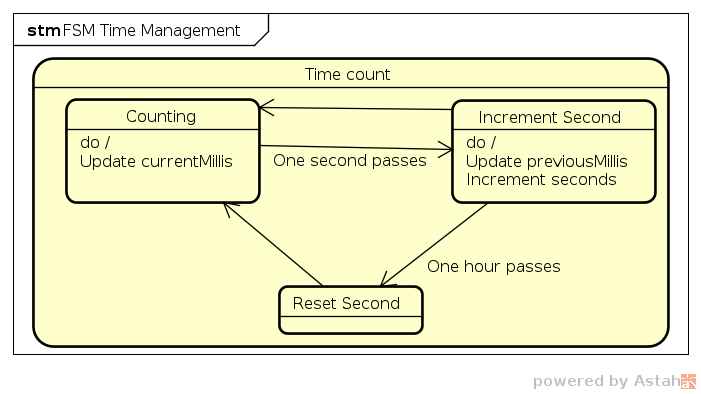
\includegraphics[width=.7\textwidth]{diagrams/FSM_TM.png}
    \caption{A FSM shows how the time counting from periodic water cycle works}
    \label{fig:fsm_tm}
\end{figure}

This representation will be important to design the next requirements,
since we could use the time management FSM to interact with more FSMs.
So this project will be event-driven,
resembling what happens in a real-world environment.

\subsection{pH Level Control}
    If the water tank's pH level is under 6,
    the high pH water will be pumped precisely,
    until the former gets the pH between 6 and 7.
    Or else,
    if the pH reaches levels greater than 7,
    deposit the low pH water in to the tank.

\begin{figure}[h]
    \centering
    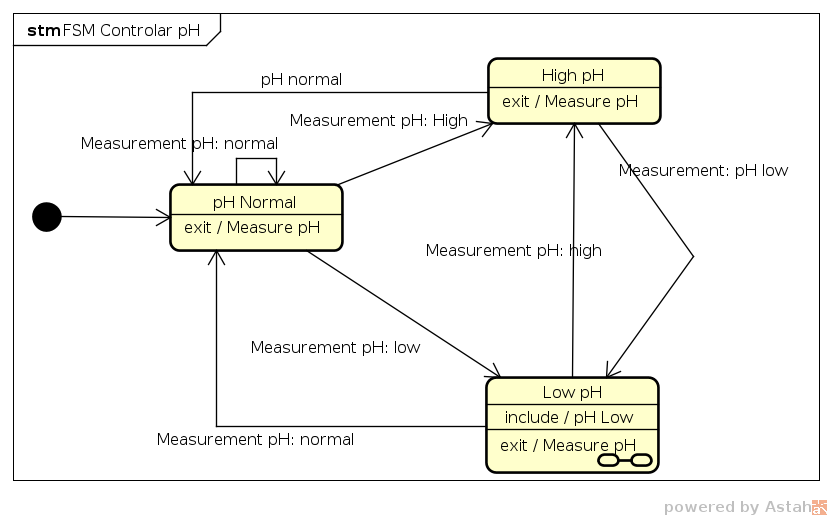
\includegraphics[width=.7\textwidth]{diagrams/pH_Control}
    \caption{A FSM to represent how the system keeps the pH at secure levels}
    \label{fig:fsm_pHc}
\end{figure}

\begin{Code}
    \centering
    \begin{lstlisting}[style=Arduino, caption=pH Control First Code, label=lst:ph1]
    /*  Keeps pH level around 6.5 */

    // Which pin is connected with the pH Sensor?
    const int pHsensorPIN = 5;
    // Which pins are connected with the pH peristaltic pumps?
    const int high_phPIN = 6;
    const int low_phPIN = 7;

    // pH Limits
    const int lowestPH = 6;
    const int highestPH = 7;

    void setup() {
        // Sets the pHsensorPIN as the output
        pinMode(pHsensorPIN, OUTPUT);
    }

    void loop() {
        pHRawValue = analogRead (pHsensorPIN);
        // Transform raw value into the actual one
        pH = process(pHRawValue);

        if ( pH < lowestPH ) {
            // Turning on the high pH pump
            digitalWrite ( high_phPIN, HIGH );
            // Guaranteeing that the low pH pump is off
            digitalWrite ( low_phPIN, LOW );
        }
        else if ( pH < highestPH ) {
            // Turning on the high pH pump
            digitalWrite ( high_phPIN, LOW );
            // Guaranteeing that the low pH pump is off
            digitalWrite ( low_phPIN, HIGH );
        }
    }
    \end{lstlisting}
\end{Code}



% Evaluation
% Related with the requirements:
% Test 1: R1: pH Control: change constant's value and verify control work
\section{Results and Evaluation}
\label{evaluation}
% Evaluation
% Related with the requirements:
% Test 1: R1: pH Control: change constant's value and verify control work


\section{Conclusion}
\label{conclusion}
% Which were the difficulties?
% Is there any POC?
% What is the contribution of this work?

As the author of this work did not have the enough experience with microelectronics,
because he had been doing the software-biased modality of his degree,
he had some difficulties relating the schematics designs,
how to use relays and other advanced components.

There are three main contributions provenient from this work: 
simple automatization of a relevant system with inexpansive components,
a documented project based on variations of a classic development model and engineering abstractions,
and a simple GUI to detail what happens with each component when the automatization happens.

The latter contribution serves as the high-level demonstration of the POC,
evincing that the use cases are being respected by simulating the sensor's value in real-time.

In the interface's aspect,
due to the communication protocol,
it is feasible to extend this system to respond to the new use cases,
such as automatic fish feeding,
solar illumation simulation,
temperature control and root cloging prevention.
The modification needed in this case is just new commands to treat new sensors inputs and outputs.


\section{Future Work}
\label{future}
\input{future}

% \section{State of Art}
% \label{sec:state_of_art}

% There are some automated aquaponics projects available on the Internet,
but most of them doesn't have a reasonable good documentation.
So it has been needed to grab parts of information among every material found on Internet.
One of the best sources found was from a hackaday's post from \cite{gareth_coleman_aquapionics_2016},
which describes with decent detail how they achieved the construction of their Arduino-powered aquaponics system.

Lots of research have been done about aquaponics.
In \cite{goddek2015challenges}, the authors show high complexity problems involving mechanisms to achieve pH equilibrium for optimizing the quality of life for the fish, plants and nitro-bacterias.
Since each living component of the system lives well in a certain pH-Range.
So there is a challenge to separate the pH level by region.

\subsection{Why people are interested in Aquaponics?}

A great amount of the published projects has a commercial goal:
to make an efficient and small-sized system that can afford to produce organic products in a large scale.

On other hand,
in the \cite{goddek2015challenges} there is a try to address the sustainability aspect of the aquaponics
This aspect stands for making a low and efficient nutrient input into the system and making a minimal environment footprint.

\subsection{Differences between Hidroponics and Aquaponics}

The Hidroponics is a system that uses a nutritive water to feed the plants.
It is a inorganic system, 
where the addition of inorganic nutrients is needed and the main live component is the plant.
On the other hand, the Aquaponics is a partly-organic system \cite{},
where the fish is added to the system,
and its waste,
the ammonia,
serves as a nutrient to the plants.

The great advantage of the Hidroponics over the Aquaponics is that the last may have some issues with human diseases,
like the presence of snails with parasites in the fish tank or some water-borne disease.


% \section{Required Components}
% \label{sec:required_components}

% \begin{description}
    \item[Arduino UNO] \hfill \\
        Some project authors recommends the Arduino MEGA because of its extra GPIO pins.
        But we only have the UNO version by now.
    \item[DC Motor] \hfill \\
        A simple DC Motor can be enough for this project.
        It could be used to feed the fish periodically.

        There is a simple mechanism inspired by the video \cite{dcmotor},
        where the fish food is wrapped in a pot and rotated down just for a arbitrary short time,
        and then rotated back up.
        It can be controlled by sending electrical current timed by the Arduino.
    \item[Waterproof Temperature Sensor] \hfill \\
        This item is necessary for monitoring whether the fish's ambient is favorable for the fish.
    \item[Water Level Sensor] \hfill \\
    \item[Water Pump] \hfill \\
        Needed to give potential energy to the water flow,
        being fundamental to the water's cycle.
    \item[pH and ORP probe] \hfill \\
        pH levelling is an essential feature of the system.
        The fish, the nitro-bacterias and the plants needs to live in a specific pH-range ambient.
        With the probe,
        when the ambient is suffering with a pH decreasing,
        the system could automatically drop some amount of CaCO3 into the water to rise the pH from the fish tank,
        for example.
    \item[Relay Board] \hfill \\
        Some items,
        like the Water Pump,
        draws too much current if compared with Arduino's capacity.
        So one needs to use relays to connected another power source with the Arduino's output signals.
\end{description}


% \section{Proof of Concept}
% \label{sec:proof_of_concept}

%% The initial idea is to make a emulated system as a proof of concept of the aquaponics system automatization.
There are some softwares that can help the project to achieve its goals.

List of softwares:
\begin{description}
    \item[Autodesk 123D Circuits] \hfill \url{http://123d.circuits.io/} \\
        \begin{verse}
            Simulate and program Arduino and breadboard components.
            Test your Arduino code in our real-time simulation environment and see your designs come to life in the browser.
        \end{verse}
    \item[Node-RED] \hfill \url{http://nodered.org/} \\
        \begin{verse}
            Node-RED is a tool for wiring together hardware devices, APIs and online services in new and interesting ways.
        \end{verse}
    \item[Fritzing] \hfill \url{http://fritzing.org/home/} \\
        \begin{verse}
            Fritzing is an open-source hardware initiative that makes electronics accessible as a creative material for anyone. We offer a software tool, a community website and services in the spirit of Processing and Arduino, fostering a creative ecosystem that allows users to document their prototypes, share them with others, teach electronics in a classroom, and layout and manufacture professional pcbs.
        \end{verse}
\end{description}



\nocite{useCaseStyle}
%\printbibliography

\end{document}
